\documentclass[a4paper,12pt]{article}

\usepackage[utf8]{inputenc}
\usepackage[T1]{fontenc}
\usepackage{graphicx}
\usepackage{color}
\usepackage{amsmath}
\usepackage{amsfonts}
\usepackage{amssymb}
\usepackage{multicol}
\usepackage{eurosym}
\usepackage{bbm}
\usepackage[french]{babel}
\usepackage{lastpage}
\usepackage{float}
\usepackage{upgreek}
\usepackage{verbatim}
\usepackage{moreverb}
\usepackage{listings}
\usepackage{textcomp}
\usepackage[nottoc]{tocbibind}
\usepackage{hyperref}
%\usepackage{subfigure}
\usepackage{subcaption}
\usepackage{ulem}
\usepackage{etoolbox}

\definecolor{color_caption}{rgb}{0.3,0.3,0.3}
\definecolor{color_section}{rgb}{0.9,0,0}
\definecolor{em_orange}{rgb}{0.9686,0.5765,0.1137}
\definecolor{em_pink}{rgb}{0.9294,0.0078,0.5490}
\definecolor{em_blue}{rgb}{0.1412,0.6667,0.8824}
\definecolor{em_green}{rgb}{0.5451,0.7765,0.2431}

\usepackage{caption}
\usepackage[font={color=color_caption},figurename=Figure,labelfont={it}]{caption}

\lstset{
language=C,basicstyle=\normalsize,upquote=true,aboveskip={1.5\baselineskip},columns=fullflexible,showstringspaces=false,extendedchars=true,breaklines=true,showtabs=false,showspaces=false,showstringspaces=false,identifierstyle=\ttfamily,keywordstyle=\color[rgb]{0,0,1},commentstyle=\color[rgb]{0.133,0.545,0.133},stringstyle=\color[rgb]{0.627,0.126,0.941},}

\DeclareMathOperator{\G}{G}

\renewcommand{\arraystretch}{1.5}
\renewcommand{\baselinestretch}{1.5}

\textheight 255mm
\headheight 15mm
\oddsidemargin -10mm
\evensidemargin -10mm
\marginparwidth 5mm
\topmargin -20mm
\textwidth 185mm
\headsep 5mm
\footskip 10mm


\usepackage{fancyhdr}

\pagestyle{fancy}

\renewcommand{\headrulewidth}{2pt}
\renewcommand{\headrule}{\hbox to\headwidth{\color{em_orange}\leaders\hrule height \headrulewidth\hfill}}
\fancyhead[L]{ENSEIRB-MATMECA}
\fancyhead[C]{Projet avancé SE}
\fancyhead[R]{E3}

\renewcommand{\footrulewidth}{2pt}
\patchcmd{\footrule}{\hrule}{\color{em_orange}\hrule}{}{}
\fancyfoot[C]{\thepage}

\usepackage{eso-pic}
\newcommand\BackgroundPic{%
\put(0,0){%
\parbox[b][\paperheight]{\paperwidth}{%
\vfill
\centering

\includegraphics[scale=0.6,%
keepaspectratio]{background}%
\vfill
}}}


\begin{document}
\parindent=1cm
\everymath{\displaystyle}
%
\AddToShipoutPicture*{\BackgroundPic}
%
\thispagestyle{empty}
%
%
\noindent
Cédric DUMONDELLE\hfill{E3}\\
Lucas FILLON\\
Xavier MARINO\\
Pierre OLIVIER\\
%
\\
%
\vspace{5.5cm}
{\color{white}t}\\
%
{\color{em_orange}\rule{\linewidth}{2pt}}
%
\textbf{{
\begin{center}
\Huge Projet avancé SE\\
%\vspace{0.6cm}
\end{center}
}}
%
{\color{white}t}\\
{\color{em_orange}\rule{\linewidth}{2pt}}\\

\vspace{9.5cm}

%
Yannick BORNAT \& Bertrand LE GAL
% \begin{tabular}{rcl}
% Dominique Dallet\hspace{4cm}\vphantom{e}&
% Professor Izzet Kale\hspace{4cm}\vphantom{e}&
% Saumya Reni
% \end{tabular}
% %
\ClearShipoutPicture
%
\newpage
%
\thispagestyle{empty}
\tableofcontents
%
\newpage
%%%%%%%%%%%%%%%%%%%%%%%%%%%%%%%%%%%%%%%%%%%%%%%%%%%%%
\setcounter{section}{-1}
\section{Introduction}
\subsection{Contexte}
De nos jours, nous disposons de différents moyens de conception, tous proposant des avantages et des inconvénients. Certains sont plus simple à mettre en œuvre, d'autres sont plus complexe mais sont généralement la solution la plus efficace. Il faut toujours mesurer le besoin d'un projet pour choisir correctement la voie de développement à privilégier.
On peut globalement résumé les différents moyens de conception à quatre grandes famille du plus souple au plus rigide, du plus généraliste au plus spécifique: CPU, GPU, FPGA, ASIC. Cependant ces quatre familles peuvent être répartis en deux sous-parties : les solutions software (CPU, GPU) et les solutions hardware (FPGA, ASIC).\newline

Dans un projet, il existe tout un tas de contraintes, qu'elles soient temporelles, financières, juridiques, humaines, etc. Ces contraintes ne sont pas négligeable, d'autant plus à échelle industrielle ou gouvernementale\footnotemark[1] où la taille de ces projets et les moyens investis sont considérables, par conséquent il est important de bien juger de la direction à prendre dans le projet pour éviter un gaspillage de ressource. 
Par exemple pour le développement d'un lecteur multimédia à destination du grand public, on pourra se permettre l'utilisation d'un processeur qui intègre éventuellement un GPU léger. En effet pour ce type de produit on peut imaginer que le coût du produit final est une priorité. Des solutions rapides à mettre en place permettant de limiter les coûts de développement et l'utilisation de composants communs et bon marché seront alors des voies privilégié. Dans le cadre du lecteur multimédia, il est possible de négliger la latence des commandes de l'utilisateur, le nombre de fonctionnalités n'a pas besoin d'être important, l'environnement graphique n'as pas besoin d'être travaillé en profondeur, le nombre de format pouvant être lue doit être le plus important possible, etc. C'est parce que les contraintes sont souples que l'on peut se permettre de développer rapidement le produit pour le rendre disponible le plus rapidement possible à la vente. Dans cette dynamique une solution hardware type généraliste, comme un processeur éventuellement couplé à un petit GPU, est certainement suffisant car le développement de software est moins coûteux et moins chronophage que le développement de hardware, de plus il permet de rajouter facilement des fonctionnalités ou des formats utilisable à l'aide de mise à jour. 
Cependant si l'on doit développer un système plus particulier tel qu'un satellite\footnotemark[2], il peut être préférable de développer soit même le hardware. En effet dans un cadre spécifique comme celui du spatial, le coût de développement et de production n'est pas la contrainte la plus forte. La fiabilité, l'efficacité, la consommation énergétique ou même la résistance au radiations ainsi que d'autres aspects techniques vont être privilégié. Comme le projet se place dans un cadre spécial, il est préférable de développer soit même les composants grâce à la solution ASIC, afin d'avoir le contrôle sur l'ensemble des fonctionnalités implémentées, sur la rapidité du système, sa fiabilité en ajoutant de la redondance, sa consommation énergétique ou la résistance aux conditions extrêmes. Bien sûr il existe d'autres milieux où les problématique sont similaire tel que l'aéronautique, la navale...\newline

Les deux précédents exemples montrent deux extrêmes et dans la réalité les contraintes s'appliquent avec des poids plus uniformisé, en effet le lecteur multimédia doit pouvoir offrir une expérience utilisateur agréable que le processeur bas de gamme n'est pas en mesure d'apporter dû à sa faible puissance de calcul et la complexité des algorithmes de compression ou d'encodage des formats multimédia, et le satellite doit tout de même respecter un budget et un temps de développement que l'ASIC ne permet pas d'honorer\footnotemark[3] à cause du coût de développement d'un masque et le temps qu'il est nécessaire pour le vérifier. Heureusement le FPGA est un entre-deux tout de même plus proche du développement hardware, il permet de s'abstraire de nombreuses problématiques onéreuse et chronophage de l'ASIC, et il permet également de fournir un soutient non négligeable à une solution généraliste en proposant un moyen d'effectuer des tâches très spécifiques plus rapidement que par le processeur ou le GPU cependant le développement et le débogage sera plus complexe.\newline

La technologie FPGA pour Field Programmable Gate Array consiste en un large réseau de porte logique, de petite mémoire, de bascule, etc, qui peuvent être connectées entre elles comme on le souhaite afin de réaliser des fonctions logique plus ou moins complexe. La technologie FPGA est donc avantageuse car un FPGA est entièrement configurable, performant et peu coûteux lorsque l'on ne souhaite pas produire en grandes quantités. Le FPGA est plus intéressant pour effectuer des tâches complexes particulières et plus intéressant que l'ASIC d'un point de vue temps et coûts de développement.\newline 

Pour configurer un FPGA, différents langages ont étaient développés permettant de décrire les fonctions logiques que l'on souhaite implémenter dans le FPGA. Celui qui nous intéresse se nomme le VHDL mais le principe est similaire avec les autres langage de la même famille tel que le Verilog. Ce est donc un langage de description, c'est à dire que l'outil de synthèse câblera le FPGA comme il l'a été décrit en VHDL. Le niveau d'abstraction est très faible, ce qui signifie qu'il est nécessaire de s'assurer de la synchronisation entre les différentes étapes d'un process, du bon dimensionnement des données, de gérer les cas particuliers d'une opération... Ce niveau d'abstraction permet une précision chirurgicale très intéressante pour des petits systèmes mais qui peut vite devenir complexe lorsque le projets devient important. Les principaux défauts de ce langage sont les suivants :\newpage
\begin{itemize}
\item[•] Il est complexe à appréhender, notamment pour des programmeurs ;
\item[•] Il est élitiste, peu de personnes connaissent et sont à l'aise avec ce langage ;
\item[•] Il est exigeant, une erreur dans la description est la synthèse pour donner un résultat non fonctionnel difficile à corriger ;
\item[•] Une description fonctionnelle est difficile à modifier sans créer de nouvelles erreurs et sans perdre de temps.
\end{itemize}

Au début le VHDL était la seule solution pour développer sur FPGA, mais depuis une dizaine d'année un nouveau langage est apparu : le SystemC. La taille des FPGA est devenue vraiment importante alors logiquement les projets devinrent important eux aussi. Il devenu courant de parler d'implémentation sur FPGA de processeur, de décodeur vidéo multi-format, de récepteur ethernet, etc. Mais avec le VHDL il devient très vite fastidieux de développer de tel projet, c'est dans ce but que le SystemC à était créé. Le principe étant de réduire le temps de développement en proposant un niveau d'abstraction plus haut que le VHDL. Ainsi il est possible de décrire du hardware tout en faisant abstraction de notion très bas niveau. C'est un langage basé sur le C++ donc plus simple à appréhender pour des programmeurs et des informaticiens, cela rompe l'élitisme du VHDL. La nature haut niveau et orienté objet de ce langage le rend plus flexible et plus facile à corriger. Le SystemC apporte différents niveaux d'abstractions grâce, entre autres, à des types plus ou moins précis, cela permet de simuler rapidement un concept et de l'affiner par la suite. Évidemment on perd la maîtrise sur la synthèse et il est difficile de savoir comment l'outil à synthétisé notre système. On perd en contrôle sur l'optimisation également, le SystemC ne permet pas d'être aussi précis qu'en VHDL mais il est possible de s'y approcher. 

%     fpga = pratique, configurable, performant et peu couteux
% vhdl = compliqué, exigeant, peu modifiable, rigide, groupusculaire (élitiste). (éviter les comparaisons vhdl/SystemC dès cette partie)
% systemC =  basé sur C++ donc accessible, mou (!= rigide), différent niveau d’abstraction pour prototypage rapide

\footnotetext[1]{les projets type gouvernementaux ou mondiaux comme la conception d'un télescope, d'une fusée, d'une station spatiale, d'un rover martien, des projets massif mais presque unique qui sont pas a visé d'un industrialisé}
\footnotetext[2]{j'ai hesité a rajouté low-cost :)}
\footnotetext[3]{je suis pas sur de cette phrase}

\subsection{Problématique}

Dans le cadre de ce projet, nous allons chercher à comparer les possibilités du SystemC par rapport au VHDL. Nous allons développer une chaîne de traitement de signaux biologiques permettant de détecter l'activité de cellule du corps. Cette chaîne de traitement à déjà était implémenté en VHDL par monsieur Bornat. \newline
Notre problématique sera donc la suivante : Quel sont les avantages du SystemC par rapport au VHDL dans le développement d'un système complexe ?  
Que permet l’utilisation du systemC par rapport au VHDL dans le cadre du développement d’un système complexe ? 
%     On a une chaîne de filtrage actuellement implémentée en vhdl, il faut tout refaire
%     Que permet l’utilisation du systemC par rapport au VHDL dans le cadre du développement d’un système complexe ? 
%     Abstraction de difficulté technique (taille de données, calcul flottant…), possibilités de tester plus rapidement différentes solutions, montrer la difficulté a débugger une implémentation
\newpage
\section{Présentation du cas d'étude}
\subsection{Introduction}
Afin de mener à bien cette étude nous nou sommes basés sur les travaux de Yannick Bornat. En effet, dans le cadre de l'analyse de signaux biomédicaux, ce dernier a mis au point un module de détection d'activité de cellules biologique, en VHDL.\\

Dans le cas de signaux provenant de cellules biologiques, l'activité cellulaire peut être détectée par un pic d'amplitude, celui-ci est représenté en figure XX. Cependant ce type de signaux possède une composante en bruit basse fréquence très élevée, c'est pourquoi il doit être filtré en amont. C'est ce signal filtré qui est utilisé à la détermination d'une valeur de seuil nécessaire à la détection d'activité biologique. Ce principe de fonctionnement, qui sera à la base du développement de notre module, est illustré en figure XX.\\

\begin{figure}[H]
\centering
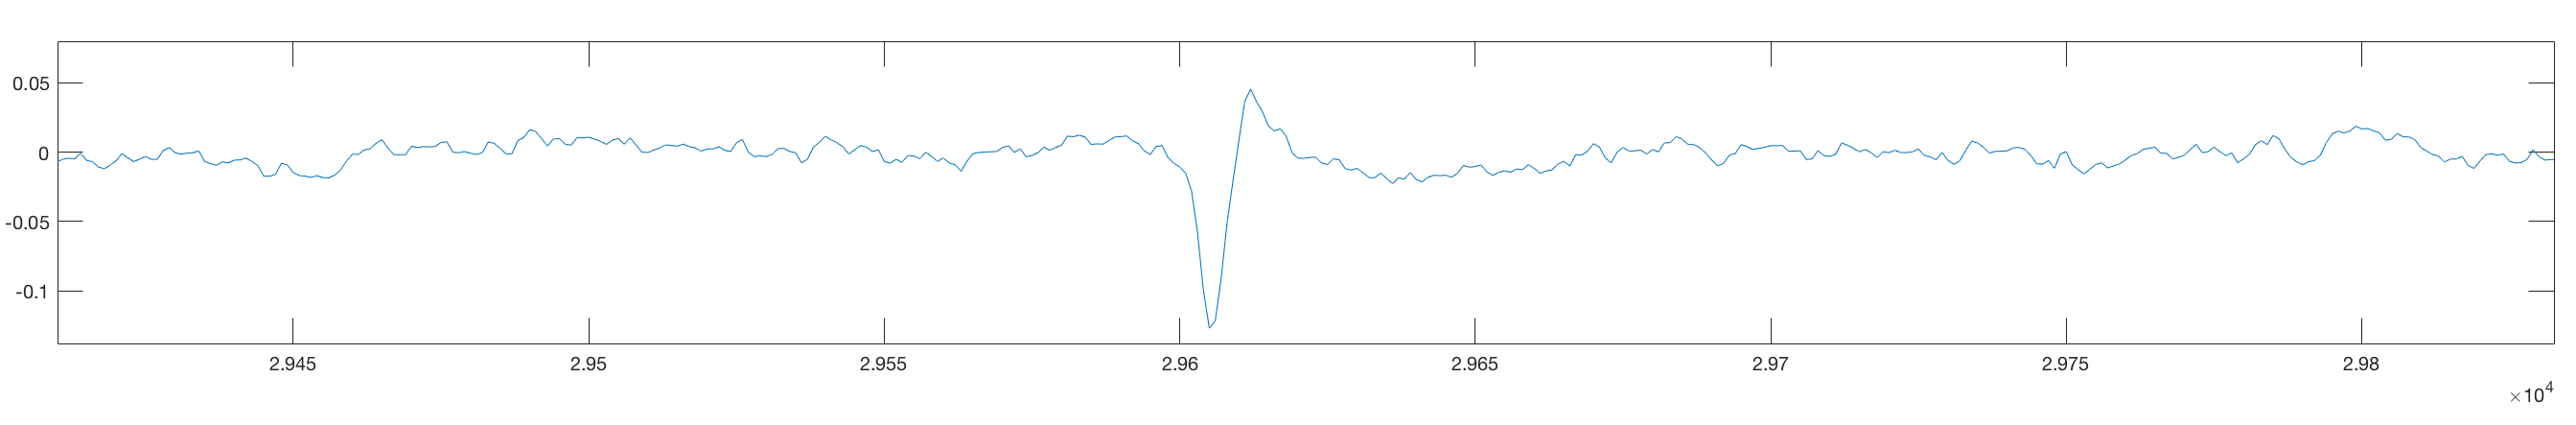
\includegraphics[scale=0.18, keepaspectratio]{toto3.png}
\caption{\textit{Pic d'activité dans un signal biologique}}
\end{figure}

\begin{figure}[H]
\centering
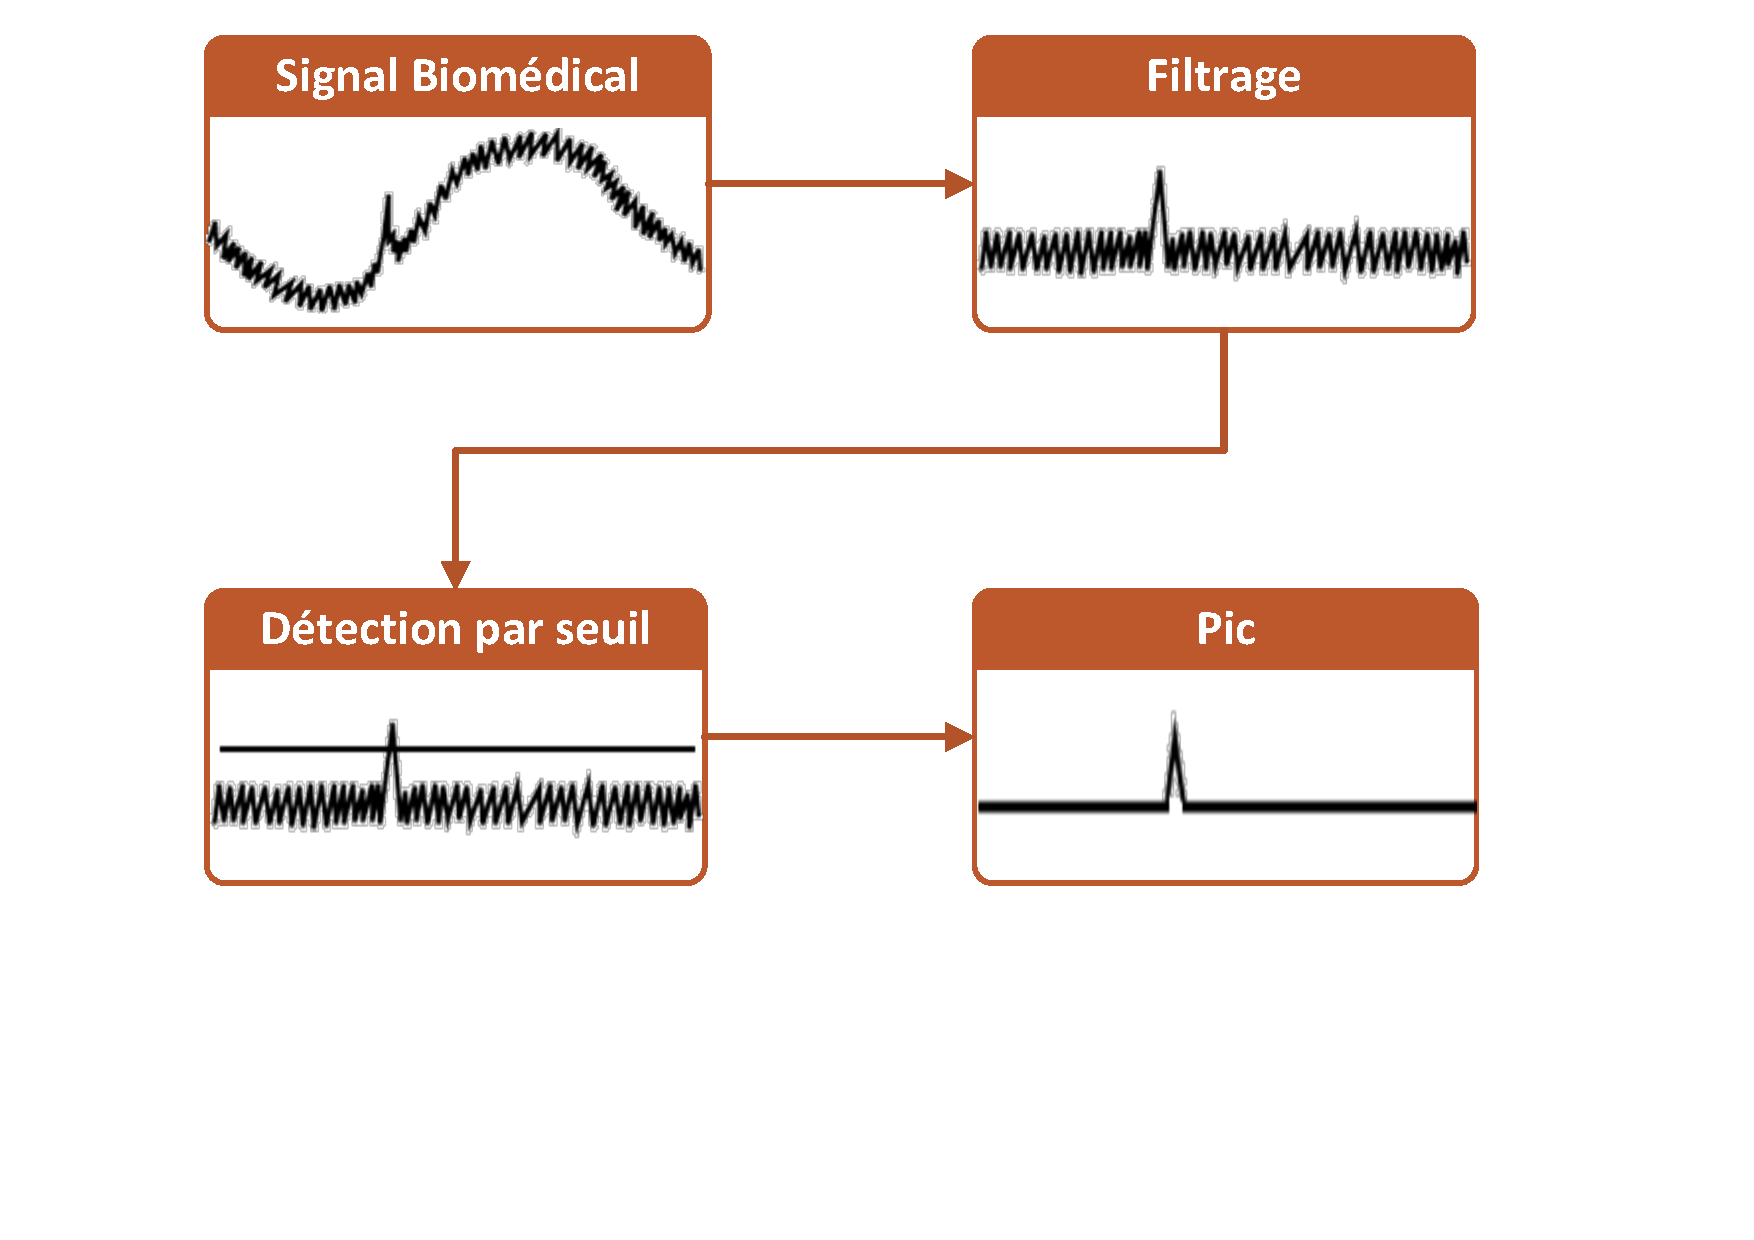
\includegraphics[scale=0.5, keepaspectratio]{Dessin1.pdf}
\caption{\textit{Principe de fonctionnement du module de détection d'activité cellulaire}}
\end{figure}
\newpage

\subsection{Fonctionnement des différents blocs}
Comme énoncé précédement, les signaux issus de capteurs biologiques sont très fortement bruité en basse fréquence, ceci se caractérise par une forte variation de l'amplitude du signal. Cette variation d'amplitude, illustrée en figure XX a) sur 5000 échantillons, est du même ordre, voir plus grand, que les que les pics attestant d'une activité celllulaire. Il convient donc de supprimer ce bruit afin de correctement détecter les pics d'activité.\\

\begin{figure}[H]
\centering
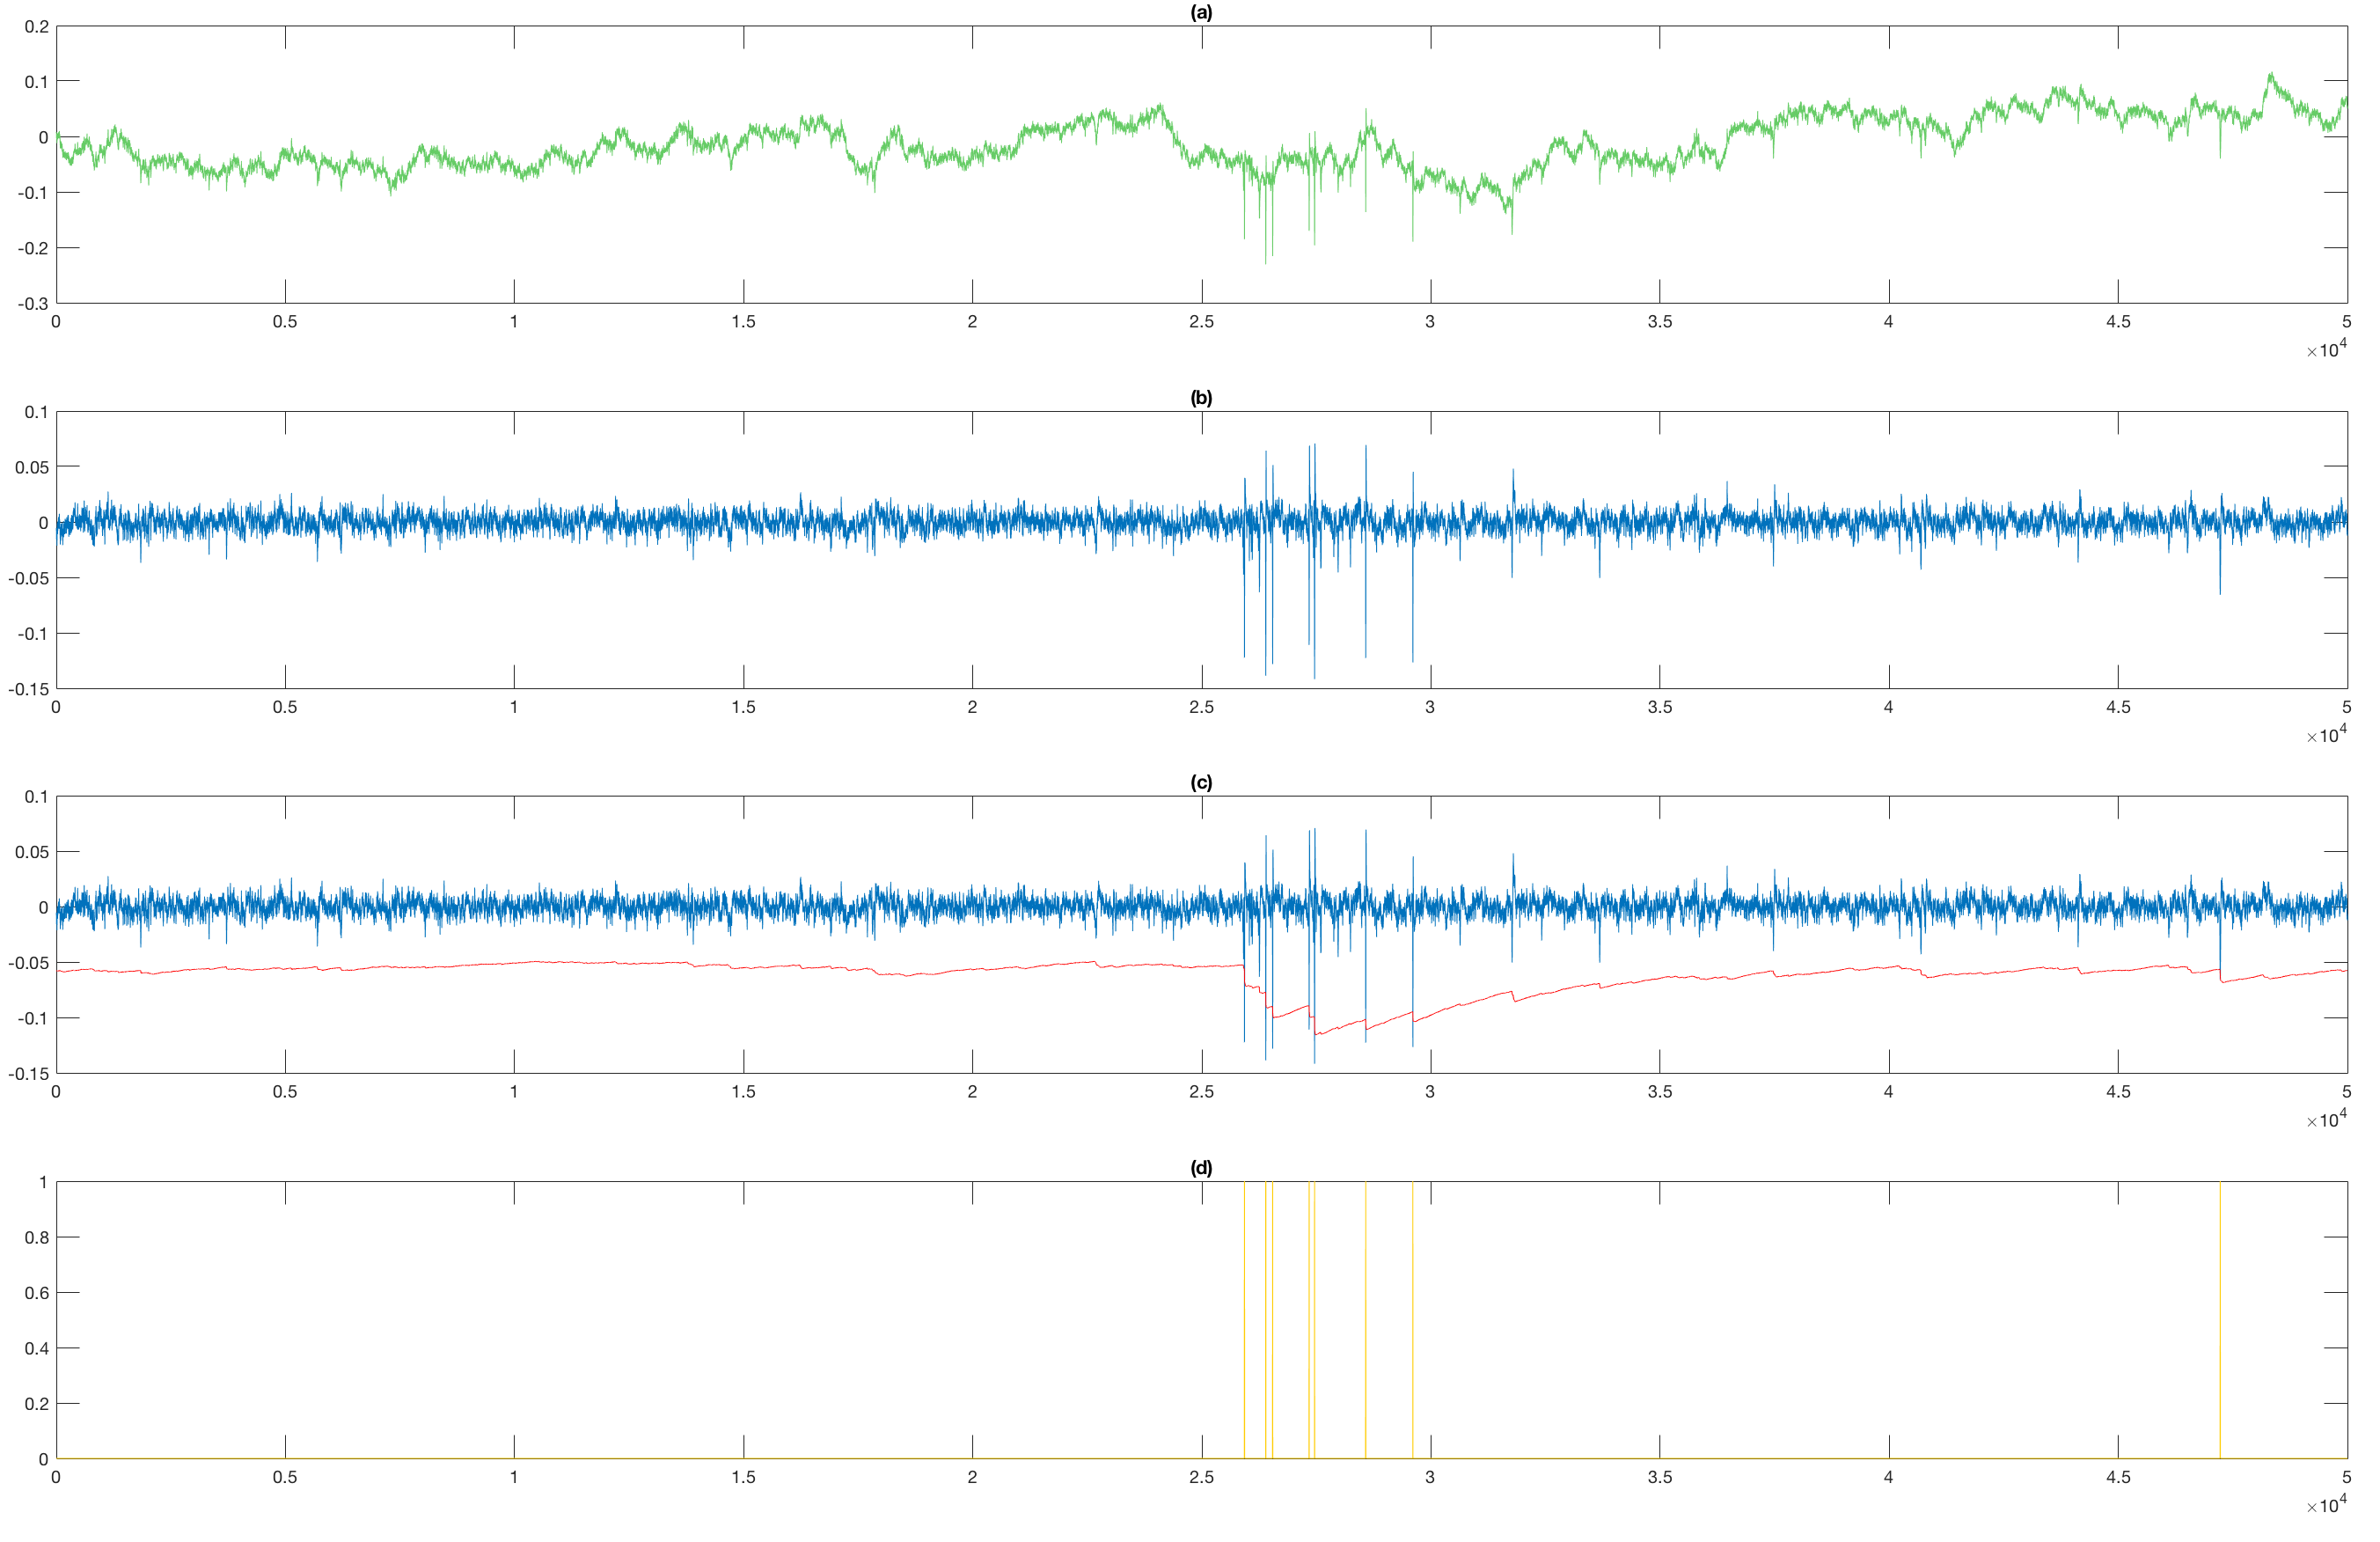
\includegraphics[scale=0.18, keepaspectratio]{toto2.png}
\caption{\textit{Évolution du signal au cours des différentes étapes de filtrage, sur 5000 échantillons}}
\end{figure}

\begin{itemize}
\item[•] \textbf{Suppression du bruit basse fréquence contenu dans le signal d'entré} : c'est un filtre passe-haut à réponse impulsionnelle infinie (IIR) qui est utilisé pour s'affranchir des basses fréquence, suivant l'équation (1).
\begin{eqnarray}
y_n = \frac{63}{64}\left(x_n - x_{n-1}\right) + \frac{31}{32}y_{n-1}
\end{eqnarray}
Le résultat issus de cette première étape de filtrage est illustré en figure XX b), on retrouve les pics caractéristiques du signal, mais celui-ci est désormais centré sur 0. On peut, cependant, constater que ce signal est également bruité en haute fréquence. C'est pour limiter l'impact de ce bruit, qu'une valeur de seuil adaptative est utilisée afin détecter les pics.\\

\item[•] \textbf{Calcul de la valeur de seuil} : deux modèles différents ont été explorés lors de cette étape, l'un d'entre eux reprennant les travaux de Yannick Bornat en appliquant une boucle de correction sur le signal d'entré filtré, tandis que l'autre méthode utilise la valeur d'écart type, de nouveau appliqué au signal filtré, (à un facteur de proportionnalité près), comme valeur de seuil.\\

\begin{itemize}
\item[\textbf{a)}] \textbf{Calcul du seuil par boucle de correction} :
\begin{figure}[H]
\centering
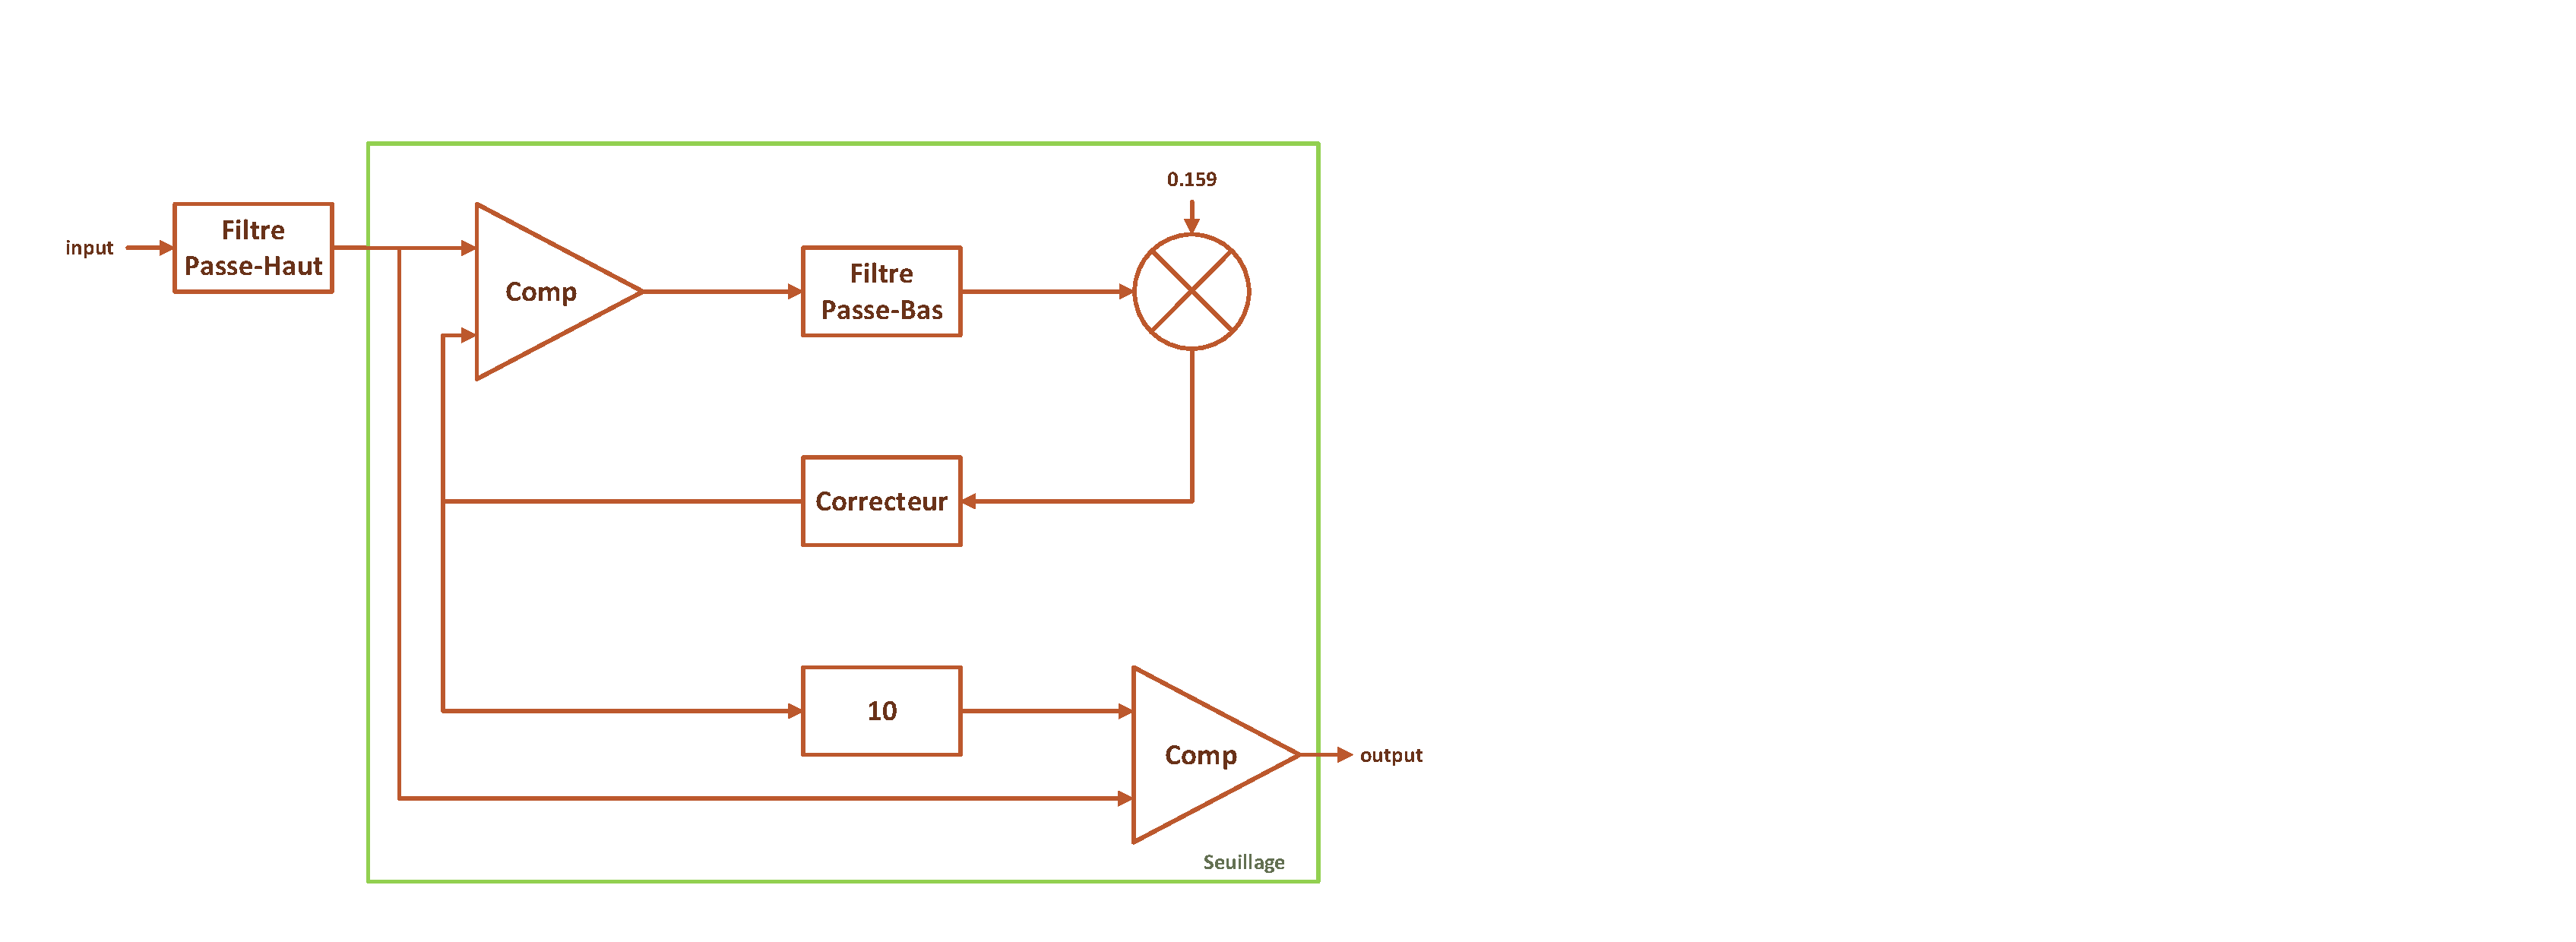
\includegraphics[width=\textwidth, keepaspectratio]{chainCedric.pdf}
\caption{toto}
\end{figure}
\item[\textbf{b)}] \textbf{Calcul du seuil par écart type} : dans cette méthode, le calcul de la valeur de seuil est assimilé au calcul de l'écart type du signal d'entré filtré. On a donc, pour une distribution uniforme des échantillons :
\begin{eqnarray*}
S = \sqrt{\frac{\sum^N_{i=1}\left(x_i-\overline{x}\right)^2}{N}},
\end{eqnarray*}
or dans notre, comme il a été souligné plus tôt, la valeur moyenne du signal a été ramenée à 0 grâce à la première étape de filtrage, on obtient donc :
\begin{eqnarray*}
S = \sqrt{\frac{\sum^N_{i=1}x_i^2}{N}}.
\end{eqnarray*}
Enfin, la fonction $x_n\mapsto\frac{\sum^N_{i=1}x_i}{N}$ a été réalisé à l'aide d'un filtre passe-bas à réponse impulsionnelle infinie, suivant l'équation (2). Les facteurs de ce filtre a on été dimensionné afin de ciblé le bruit en haute fréquence du signal.
\begin{eqnarray}
y_n = \frac{1}{524288}\left(x_n + x_{n-1}\right) + \frac{2047}{2048}y_{n-1}
\end{eqnarray}
La valeur de seuil ainsi obtenue est illustrée par la courbe rouge de la figure XX c). Une fois la valeur de seuil déterminée, celle-ci est utilisée comme référence afin de détecter les pics présents dans le signal d'entré filtré, comme
 l'illustre la figure XX d). On peut retrouver le schéma du principe de la fonction de seuillage en figure XX.
\begin{figure}[H]
\centering
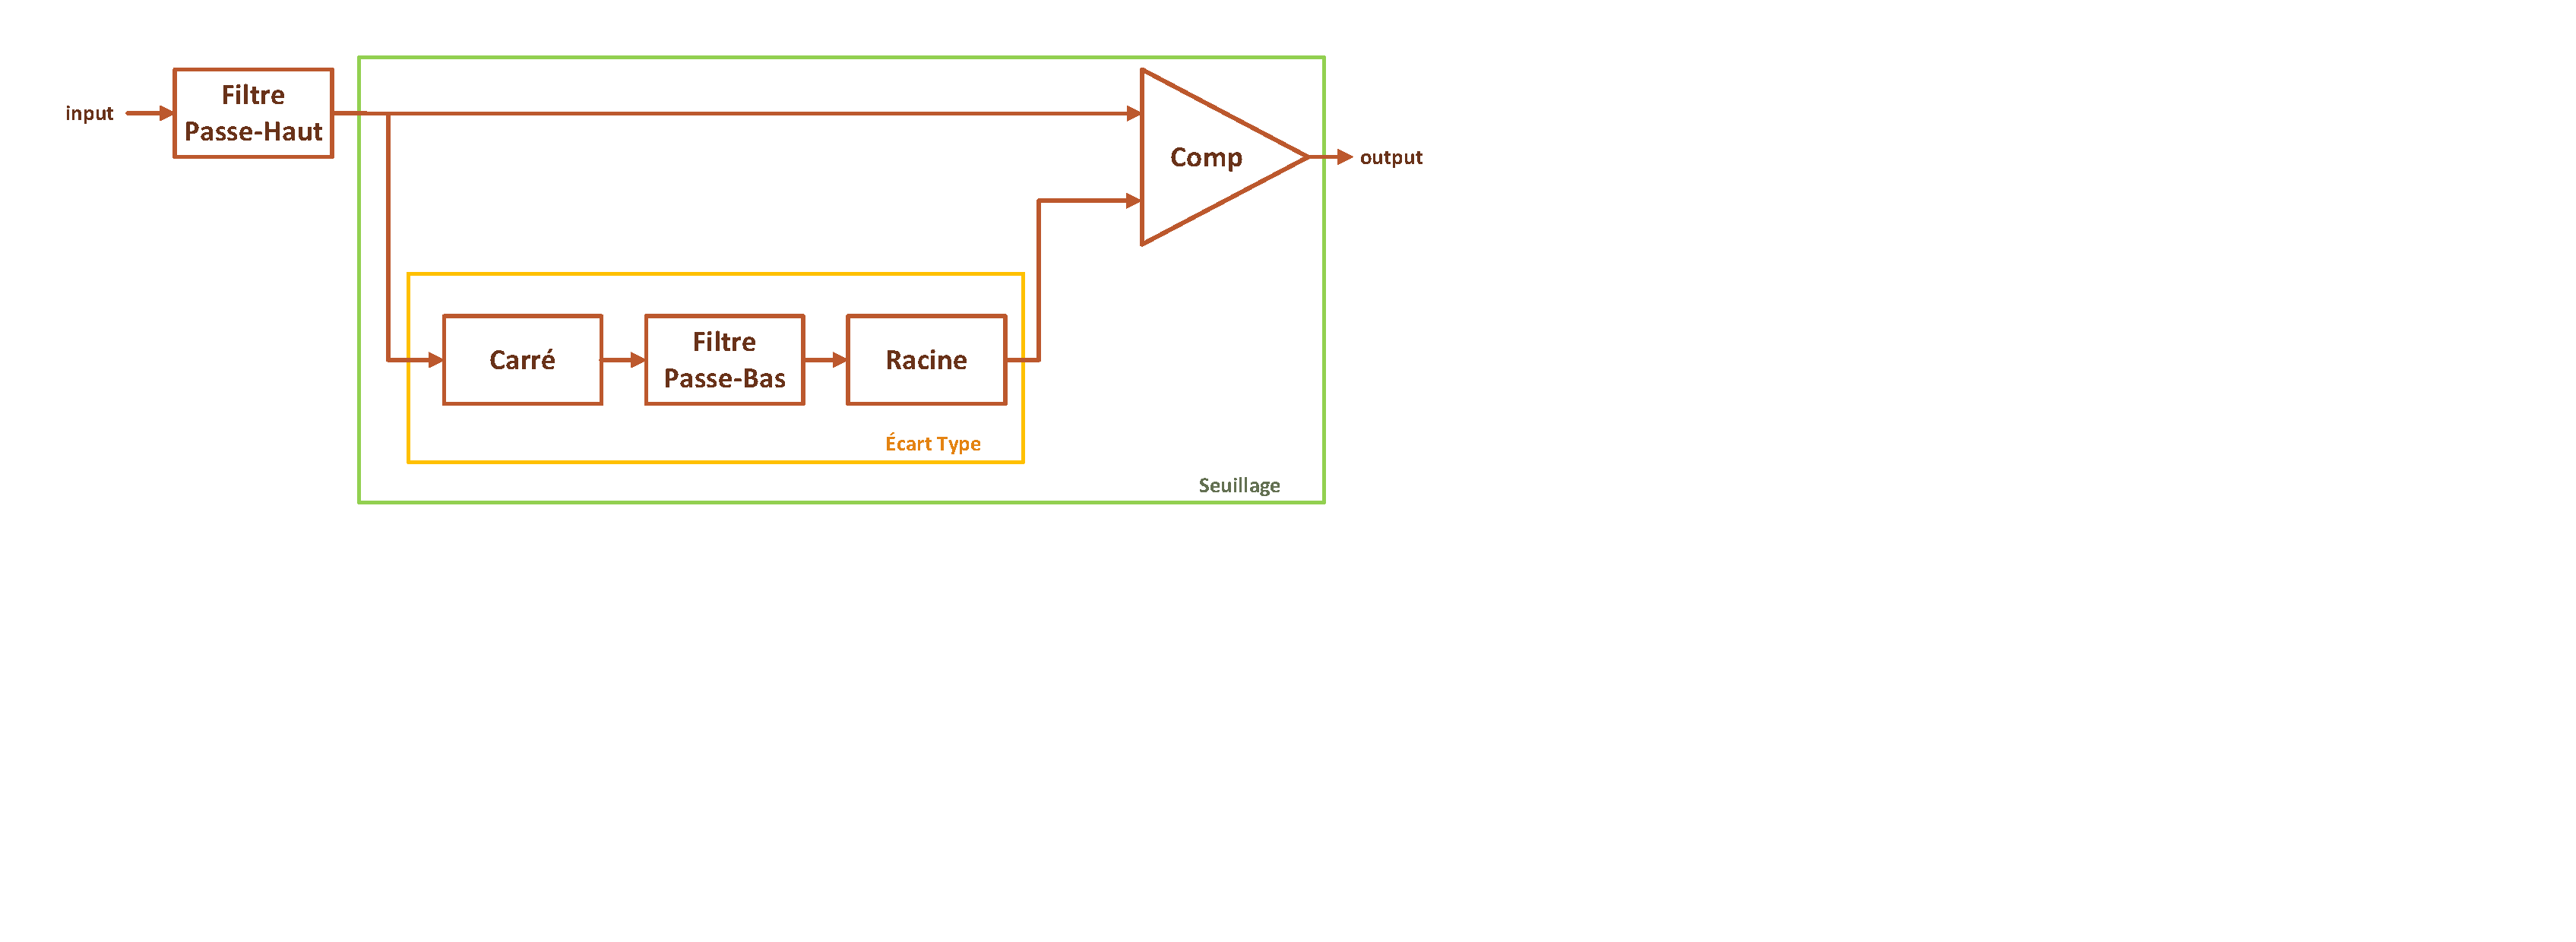
\includegraphics[width=\textwidth, keepaspectratio]{chainXavier.pdf}
\caption{Schéma de principe du calcul de l'écart type}
\end{figure}
\end{itemize}
\end{itemize}
\newpage
\section{Implémentation depuis le SystemC}
	Les schémas présentés en Figures X et X permettent de se représenter le fonctionnement de la chaîne globale. La modularité du SystemC nous permet alors de concevoir une paire de fichiers, un fichier source de description ainsi qu'un \textit{header}, pour chacun des blocs composant ces schémas. Il convient de détailler le cheminement suivi à partir de la création de ces fichiers jusqu'à leur implémentation sur la carte Nexys 4. Cette partie vient donc présenter le flot de conception/compilation lié au SystemC et sa mise en œuvre lors du projet.

\subsection{Flot de compilation}
	L'apprentissage d'un nouveau langage de description ou de programmation passe nécessairement par la compréhension du flot de compilation qui lui est associé. Pour le SystemC, on peut découper ce flot en quatre étapes principales illustrées par la Figure X :
	\begin{figure}[H]
		\centering
		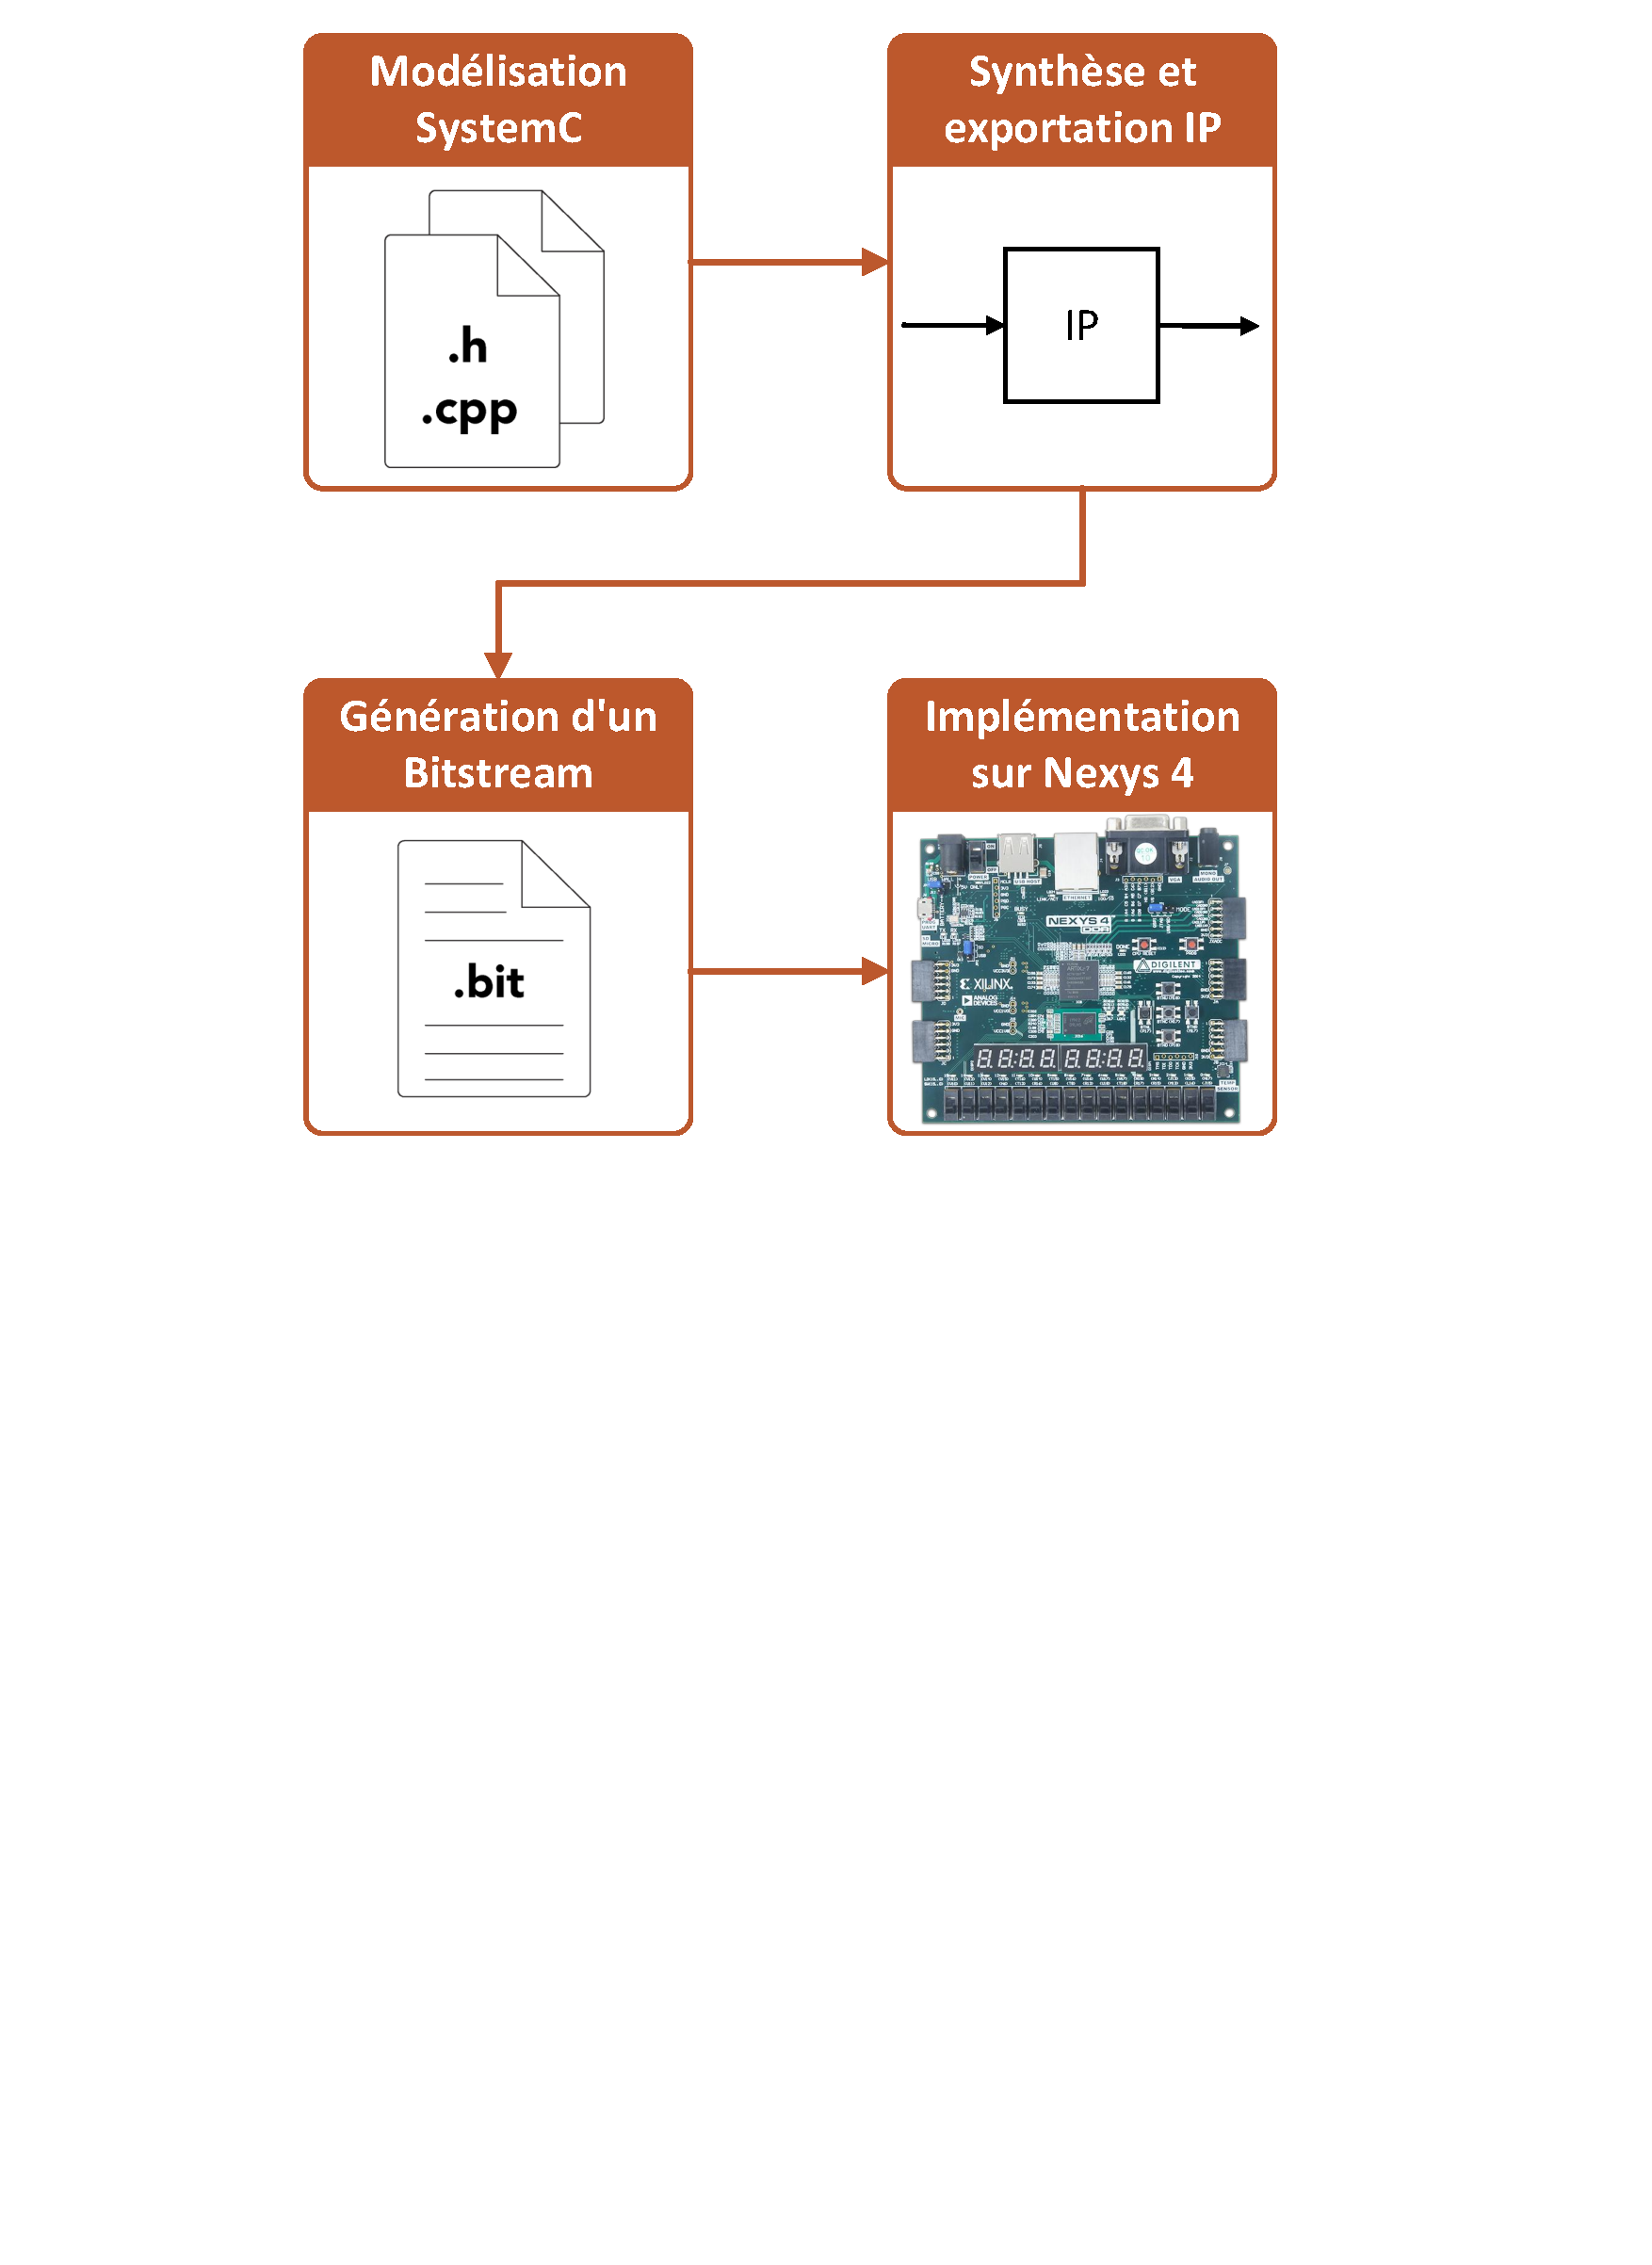
\includegraphics[scale=0.5, keepaspectratio]{Dessin2.pdf}
		\caption{Flot de compilation}
	\end{figure}
	\begin{itemize}
		\item[\textbullet] \textbf{Modélisation SystemC} : dans un premier temps il convient de décrire en SystemC le système que l'on souhaite modéliser. Pour cela, on rédige des fichiers sources \sout{dans un IDE} SystemC pour symboliser chacun des blocs décrits précédemment. \\
		\item[\textbullet] \textbf{Synthèse et exportation IP} : une fois les fichiers SystemC écrits, on peut désormais les passer dans l'environnement \textit{Vivado HLS} afin de les synthéthiser et d'exporter un ou plusieurs blocs sous forme d'IP (\textit{Intellectual Property}). Ces blocs IP sont des blocs logiques, avec des entrées et des sorties, qui vont être implémentés sur FPGA par la suite. \\
		\item[\textbullet] \textbf{Génération d'un Bitsream} : un bloc IP ne pouvant être envoyé directement sur FPGA, il convient de l'intégrer dans un \textit{top-level}, décrit en langage VHDL, pour pouvoir notamment interfacer ses entrées et sorties avec les entrées et sorties physiques de la carte Nexys 4. Pour ce faire, l'environnement \textit{Vivado} est requis et permet de générer un \textit{bitsream} d'extension \texttt{.bit}. \\
		\item[\textbullet] \textbf{Implémentation sur Nexys 4} : finalement, le \textit{bitsream} peut être envoyé sur la carte cible, dans notre cas la carte Nexys 4, via le port série de notre ordinateur. A ce stade, les fichiers décrits en SystemC sont implémentés sur FPGA.\\
	\end{itemize}
	Le flot de compilation présenté ici allie le développement \textit{software} de sources SystemC, et l'implémentation \textit{hardware} des blocs ainsi créés. Il s'agit là du flot de compilation suivi lors du projet et les parties 2.2 et 2.3 suivantes viennent détailler sa mise en pratique.


\subsection{Modélisation en SystemC et simulations}
L'interêt d'utiliser le langage SystemC afin de décrire nos sources reposent sur la flexibilité apportée par l'utilisation d'un langage de haut niveau. En premier lieu, le SystemC possède de nombreux outils permettant la description de modules au même titre qu'un langage de bas niveau tel que le VHDL :
\begin{itemize}
\item[•] La classe \texttt{sc\_module} peut facilement être assimilé à une \texttt{entity} en VHDL, tandis que ça nature de classe lui permet d'utiliser des outils de C++ tel qu'un constructeur, \texttt{sc\_ctor}.
\item[•] Les
\end{itemize}
\subsection{Implémentation sur FPGA et validation}
	Une fois les fichiers SystemC écrits et les simulations en \textit{software} vérifiées, il convient de tester les blocs et chaînes entières en \textit{hardware}. Pour cela, un environnement de test a été mis en place et il est illustré en Figure X.
	\begin{figure}[H]
		\centering
		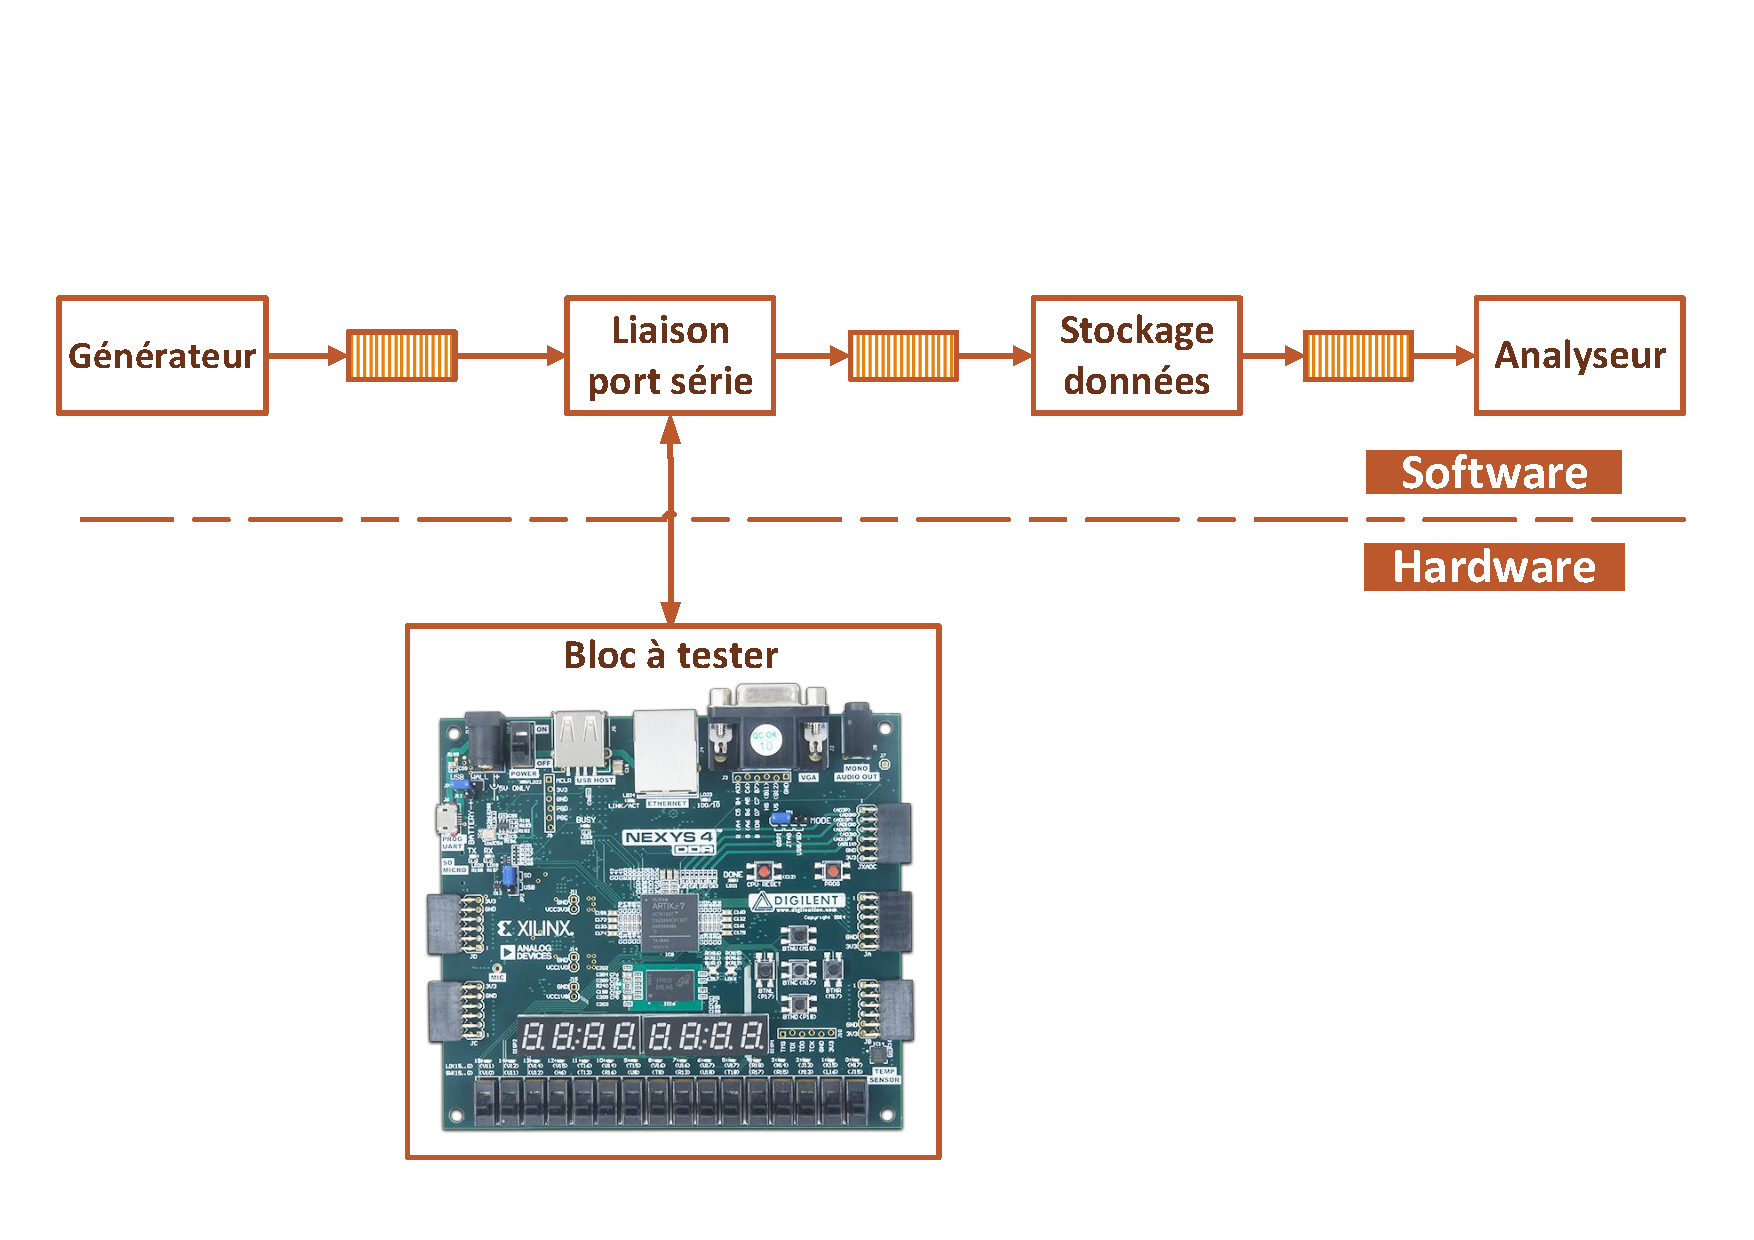
\includegraphics[width=\textwidth, keepaspectratio]{Dessin6.pdf}
		\caption{Environnement de test}
	\end{figure}
	\noindent On distingue ici deux parties essentielles :\\
	\begin{itemize}
		\item[\textbullet] la partie \textit{software} : elle se déroule sur un ordinateur, sous \textit{Vivado HLS} par exemple, et permet de lancer une simulation,\\
		\item[\textbullet] la partie \textit{hardware} : elle représente la carte Nexys 4 reliée en USB sur le port série de l'ordinateur, elle contient également l'implémentation du bloc IP à tester.\\
	\end{itemize}

	Avant de tester les chaînes globales développées en SystemC, les blocs réalisant la racine carrée ainsi que la puissance au carré ont notamment été implémentés sur FPGA. Pour ce faire, le bloc "\textit{Générateur}" permet de venir lire les données d'entrée stockées dans un fichier texte, que ce soit les valeurs extraites du signal biomédical ou bien des valeurs plus rudimentaires pour tester la racine carrée. Après passage dans une FIFO, les données sont envoyées sur le port série et traitées sur le FPGA. Ce dernier contient l'IP que l'on souhaite tester en \textit{hardware}, la racine carrée par exemple, et renvoie les données sortantes vers le bloc "\textit{Stockage données}". Ce bloc écrit alors les données calculées sur le FPGA dans un fichier texte. Comme expliqué en 2.2, les données contenues dans une FIFO doivent être consommées, c'est pourquoi le bloc "\textit{Analyseur}" se contente de venir lire dans la FIFO, pour fermer la chaîne de test.  \\ \\
	\indent En ce qui concerne l'échange de données entre la partie \textit{software} et le FPGA, le module de communication utilisant l'UART et développé par Yannick Bornat a été utilisé. Cependant, les deux chaînes précédemment décrites manipulent des données de type \textit{float}, donc sur 32 bits, tandis que l'UART ne reçoit et renvoie que des données sur 8 bits. Pour palier à cette incompatibilité, des \textit{wrappers} ont été décrit en SystemC selon le modèle présenté en Figure X. Le \textit{wrapper IN} reçoit les données provenant de l'UART sur 8 bits et les reforme sur 32 bits, en attendant donc quatre paquets de 8 bits, et les envoie ensuite au bloc de test, tandis que le \textit{wrapper OUT} fait l'opération inverse et découpe la donnée en quatre paquets de 8 bits, chacun d'eux envoyé à l'UART. De plus, le bloc "\textit{Ouverture port série}" réalise également ce découpage des données sur 8 bits en entrée et la reformation de la donnée de sortie sur 32 bits car il communique directement avec l'UART et la partie \textit{software}. Ces deux wrappers ont alors été synthéthisés et exportés en tant qu'IP avec le bloc à tester.  
	\begin{figure}[H]
		\centering
		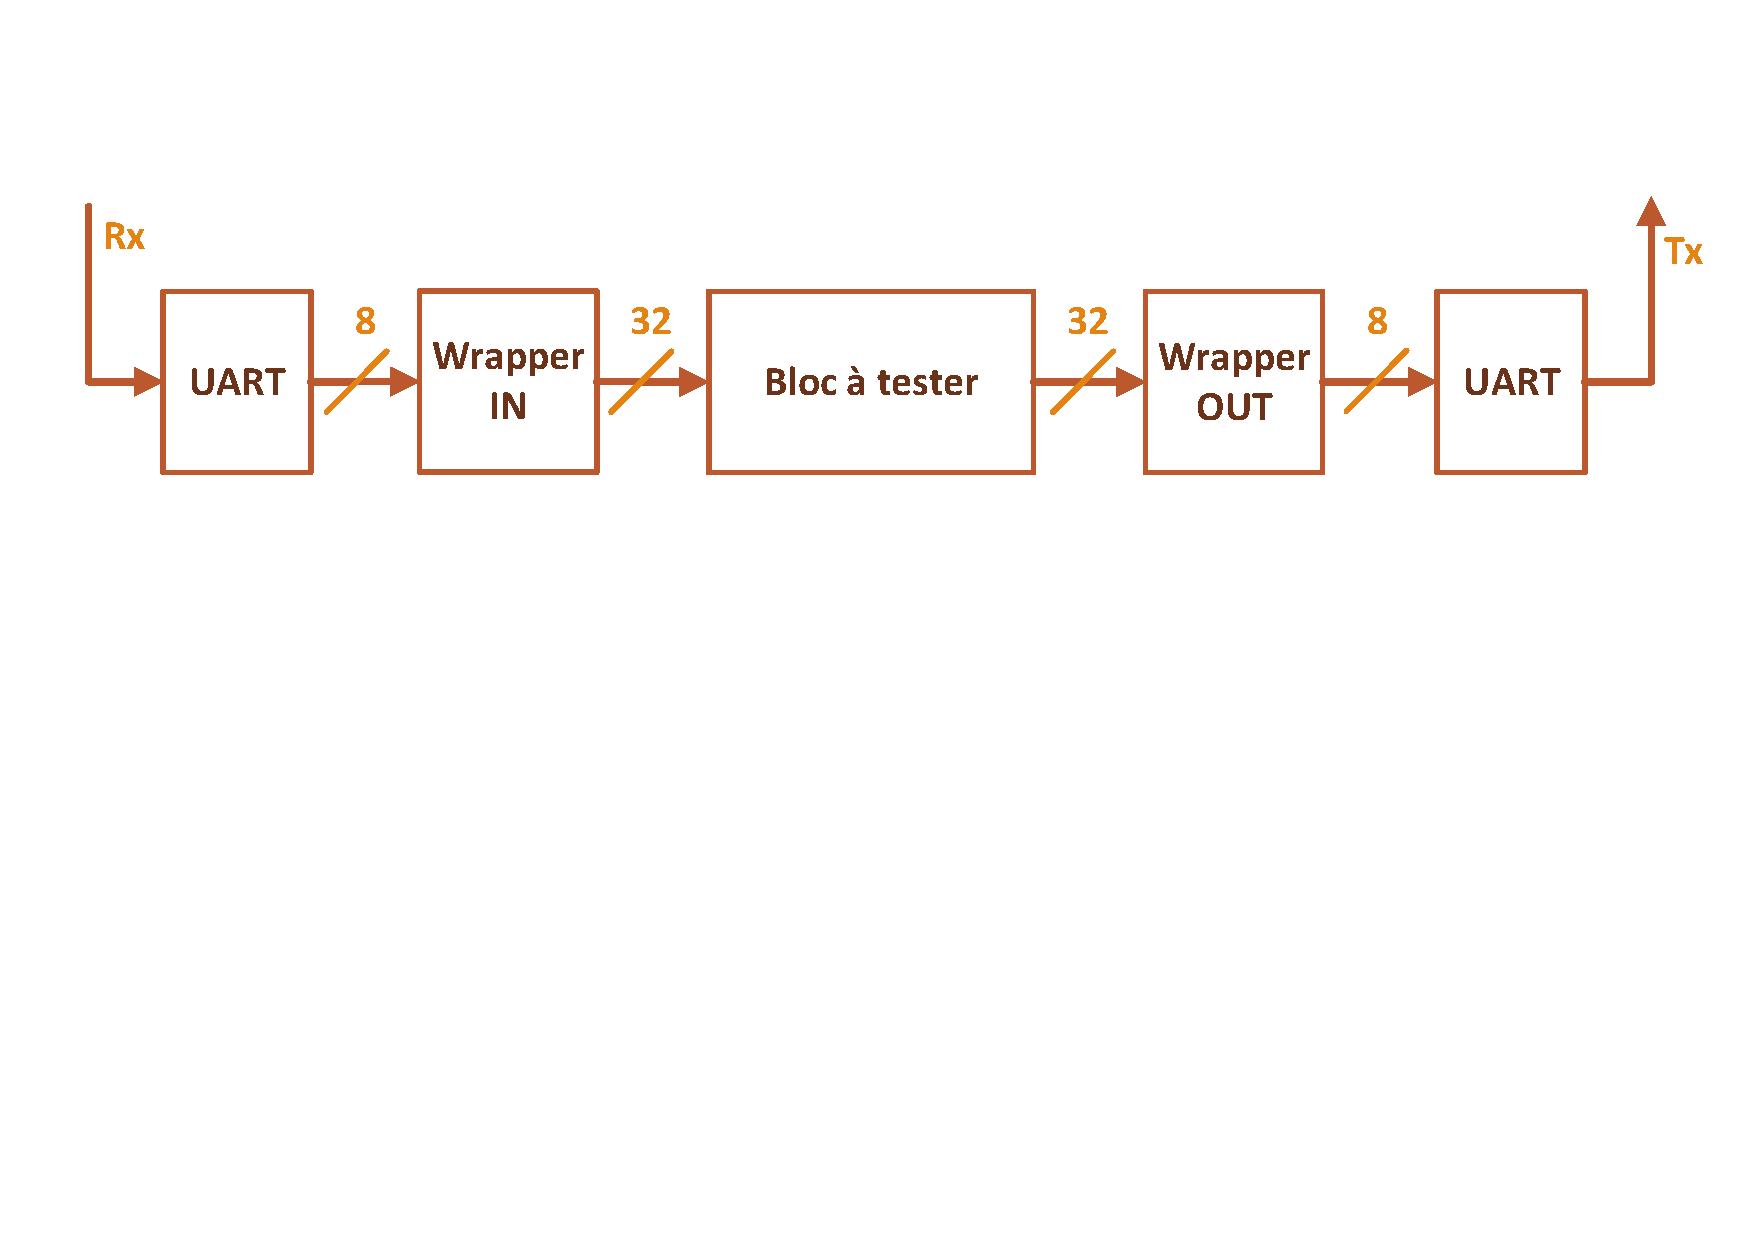
\includegraphics[width=\textwidth]{Dessin7.pdf}
		\caption{UART Wrappers}
	\end{figure}   

	Lorsque les différents blocs ont été validés un à un sur cet environnement de test, les deux chaînes ont pu successivement être implémentées sur FPGA. Leur validation est, quant à elle, passée par une comparaison entre les données traitées et celles de référence obtenues après développement en VHDL de Yannick Bornat. La principale difficulté de cette démarche d'implémentation \textit{hardware} résidait dans l'envoi et la réception des données entre la chaîne de simulation et la carte Nexys 4. En effet, le goulot d'étranglement se trouve dans la communication avec l'UART qui attend de recevoir une donnée avant d'en transmettre une autre. Une fois cette notion appréhendée il a été possible de vérifier le fonctionnement de n'importe quels blocs.
\newpage
\section{Résultats}
\newpage
\section{Conclusion}

\end{document}


